\documentclass{article}
\usepackage{amsmath,amsthm,amsfonts}
\usepackage{graphicx}
\usepackage{tikz,pgfplots}
\usetikzlibrary{positioning}


\title{Graphs - TikZ}
\author{Dark Lord}


\begin{document}
\maketitle

\section{TikZ}
0
\tikz \draw (0,0) -- (2,1) -- (3,2);

\begin{tikzpicture}
\draw (0,0) circle (1);
\draw (2,0) circle (1.5in);
\draw (5,0) ellipse (10pt and 20 pt);

\draw node at (3,0) {$f(x)$};
\filldraw (6,2) circle (0.05cm) node[anchor=west]{Anchored Node};
% anchor west means the circle is to the west of the node
\end{tikzpicture}

\vspace{1in}
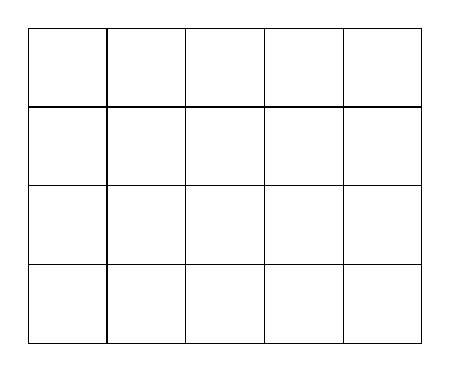
\begin{tikzpicture}
\draw (0,0) rectangle (3,4);
\draw (0,0) grid (5,4);
\end{tikzpicture}


\newpage
% Illusion of sphere
\begin{center}
    
\begin{tikzpicture}[transform canvas={scale=4.0}]

        \draw[blue] (0,1) arc (90:-90: 0.5cm and 1cm);
        \draw[red,dashed] (0,1) arc (90:270: 0.5cm and 1cm);
        \draw (0,0) circle (1cm);

        \filldraw[red] (0,1) circle (0.05);
        \filldraw[red] (0,-1) circle (0.05);
        
        \shade[ball color=blue!10!white, opacity=0.2] (0,0) circle (1cm);

    \end{tikzpicture}
\end{center}

\vspace{5cm}
% Lines of Different Thicknesses
\begin{tikzpicture}
    \draw[ultra thick] (0,3) -- (2,3);
    \draw[very thick] (0,2.5) -- (2,2.5);
    \draw[thick] (0,2) -- (2,2);
    \draw[thin] (0,1.5) -- (2,1.5);
    \draw[very thin] (0,1) -- (2,1);
    \draw[ultra thin] (0,.5) -- (2,.5)
\end{tikzpicture}

\vspace{2in}
% Flowchart

\begin{tikzpicture}[
    SIR/.style={rectangle, draw=red!60, fill=red!5, very thick, mininmum size=5mm}    
]
% we just defined the style of the node, nothing else

%Nodes
\node[SIR] (Susceptible)
\node[SIR] (Infectious)
\node[SIR] (Recovered)



\end{tikzpicture}



\end{document}

